\section{Appendix}

\begin{figure}
    \begin{center}
        %\hspace{-7mm}
        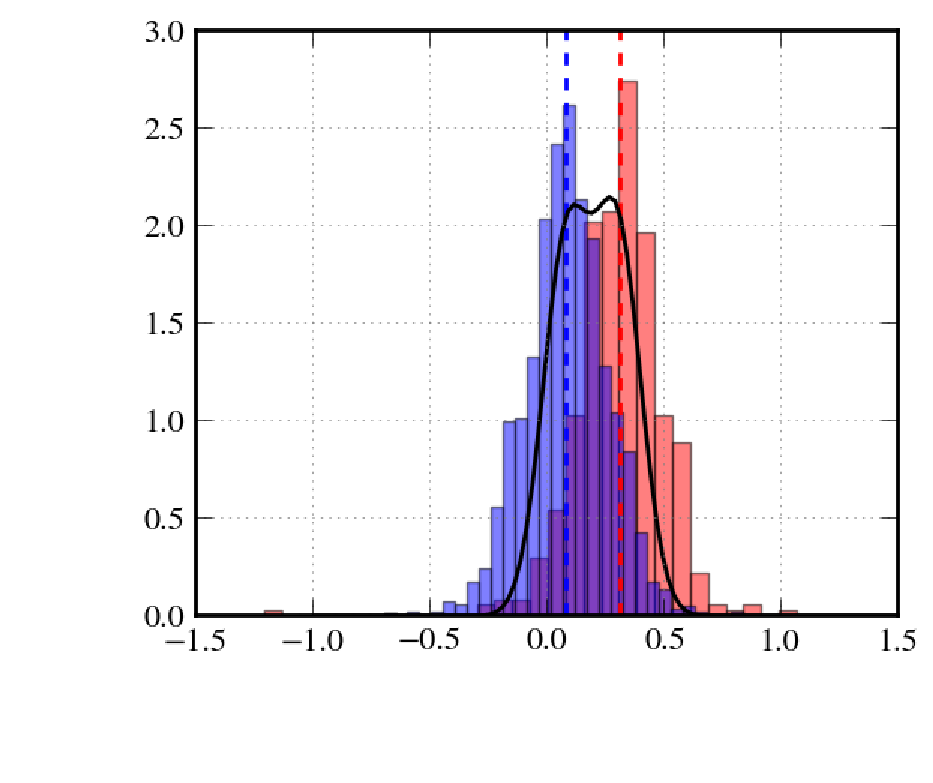
\includegraphics[width=0.5\textwidth]{fig/pymcmetals}
        \caption{Reconstruction of two populations from mock data. The
          underlying metallicity distributions are shown as red and
          blue histograms. The retrieved centers of the Gaussians are
          shown as vertical lines, and the reconstructed metallicity
          distribution is depicted as black line.}
        \label{fig:pymcmetal}
    \end{center}
\end{figure}

%%% Local Variables: 
%%% mode: latex
%%% TeX-master: "Steger+_2014_Gravlite"
%%% End: 
